\chapter{Application Features}
\label{ch:ApplicationFeatures}

%%%%%%%%%%%%%
\section{Graphical User Interface (GUI)}

\noindent
For Milestone 1, we designed the graphical user interface of the application using JavaFX and SceneBuilder. In Milestone 2, we extended this UI into a functional prototype by integrating a live SUMO connection, real-time stepping, map rendering, vehicle injection, and traffic light control. In the final milestone, we added statistical charts and graphs that visualize changing vehicle data in real time.
\medskip

\noindent
The interface is built around a \texttt{BorderPane} layout, dividing the window into clear functional regions. At the top of the application, a responsive toolbar provides the essential simulation controls, including opening a SUMO configuration file, connecting to the simulation backend, starting or pausing the simulation, executing single simulation steps, and adjusting the simulation speed. This layout remains clean and stable when the window is resized.
\medskip

\begin{figure}[H]
    \centering
    \includegraphics[width=0.8\textwidth]{Figures/main_ui_final.png}
    \caption{Final Graphical User Interface (GUI)}
    \label{fig:main-ui}
\end{figure}

\noindent
On the left side, a \texttt{TabPane} organizes settings into tabs such as Simulation, Vehicles (injection), Traffic Lights, and Filters. The Simulation tab supports selecting a \texttt{.sumocfg} file and adjusting the step interval, while the Vehicles tab provides controls for injecting vehicles into a selected edge. The Traffic Lights tab allows the user to view current status of a specific traffic light and manipulate its state as well, and the Filters tab supports viewing the map under conditional restraints.
\medskip

\noindent
The central region contains the map view. In the final milestone, this region renders the SUMO network (parsed from the network file referenced by the loaded \texttt{.sumocfg}) and draws moving vehicles, environmental background based on TraCI position updates. The map supports zooming and panning to inspect local behavior around intersections.
\medskip

\begin{figure}[H]
	\centering
	\includegraphics[width=0.8\textwidth]{Figures/map_final.png}
	\caption{Live map rendering and simulation controls in the JavaFX GUI}
	\label{fig:map-ui}
\end{figure}

\noindent
On the right side, there is a dropdown menu for exporting simulation data as a comma separated values (CSV) file or portable document format (PDF) file. A second \texttt{TabPane} provides simulation metrics. In the Map Overview tab, line chart are drawn to track vehicle count, average speed, and speed distribution over time. The Vehicle Data tab contains a JavaFX \texttt{TableView} that is populated with live data (vehicle ID, speed, current edge, and color). Detailed vehicle data is organized in a table and a pie chart of their color distribution is also shown.
\medskip

\noindent
Finally, a status bar at the bottom displays key runtime information such as simulation step, simulation time, vehicle count, and connection status.
\medskip

\begin{figure}[H]
	\centering
	\includegraphics[width=1\textwidth]{Figures/status_bar.png}
	\caption{Status Bar of the application window}
	\label{fig:status-bar}
\end{figure}

\noindent
Overall, the UI now provides a complete workflow for the application: load a scenario, connect to SUMO, run or step the simulation, visualize the network with moving vehicles, inject vehicles interactively, manipulate traffic light phases, filter vehicles by different criteria, inspect detailed metrics, and exporting simulation data to external files.
\medskip

%%%%%%%%%%%%%
\section{Core Functionalities}

\subsection{Live SUMO Connection and Simulation Control}

\noindent
The application establishes a TraCI connection to SUMO and manages the simulation lifecycle (connect, disconnect, step, and run/pause). The simulation can run continuously with a configurable step length (default is 50 ms), and the GUI reflects the current state through a status bar (step number, simulation time, and vehicle count). The UI also remembers the last opened \texttt{SumoConfig} file for express running, in case there is no need to change simulation network.
\medskip

\begin{figure}[H]
	\centering
	\includegraphics[width=0.5\textwidth]{Figures/traci_connection_select.png}
	\caption{TraCI Connection Selection Menu}
	\label{fig:traci-select}
\end{figure}

\noindent
Additionally, users can press P on the keyboard to toggle Play/Pause for the simulation.
\medskip

\subsection{SUMO Traffic Network File Organization}

\noindent
There are 5 types of files associated with each SUMO project. The \texttt{.netecfg} file keeps record of all other files in the project, mainly used for the \texttt{netedit} GUI, not necessarily for running SUMO simulations. It references the \texttt{.sumocfg} file, which is the main storage of all data for that specific simulation. The \texttt{.sumocfg} file references 3 other files:
\medskip

\begin{itemize}
	\item \texttt{.net.xml}: network data, containing data about the map, such as edges, lanes, junctions, traffic lights
	
	\item \texttt{.rou.xml}: route data, containing data about routes, traffic flows, vehicles, etc.
	
	\item \texttt{.add.xml}: additional data, containing data about bus stops, charging stations, parking areas
\end{itemize}

\begin{figure}[H]
	\centering
	\includegraphics[width=0.8\textwidth]{Figures/sumo_file_structure.drawio.png}
	\caption{SUMO Traffic Network File Structure}
	\label{fig:sumo-files}
\end{figure}

\subsection{Map Visualization in the Application}

\noindent
The map renderer parses the SUMO network file (\texttt{.net.xml}) to extract lane polylines and junction shapes. During runtime, the renderer updates vehicle positions from TraCI and draws moving vehicles on top of the network. A key feature introduced in Milestone 2 is the interactive zoom and pan capability, allowing users to inspect specific intersections or view the entire network at a glance. To improve interpretability at intersections, the map overlays traffic-light stop lines colored by the current signal state (red/yellow/green), providing immediate visual feedback on signal phases.
\medskip

\begin{figure}[H]
    \centering
    \includegraphics[width=0.8\textwidth]{Figures/zoom-in_map.png}
    \caption{Zoomed-in map view with moving vehicles and traffic-light stop-line overlays (red/yellow/green).}
    \label{fig:zoom-map}
\end{figure}

\subsection{Vehicle Injection}

\noindent
Users can inject vehicles during a running simulation by selecting a target edge and specifying the number of vehicles, an optional speed, and a vehicle color. The ability to customize vehicle color was recently added to help visually distinguish injected fleets from background traffic. Injected vehicles are immediately reflected in the map rendering and vehicle table, enabling quick scenario exploration and load testing.
\medskip

\begin{figure}[H]
    \centering
    \includegraphics[width=0.4\textwidth]{Figures/vehicle_injection.png}
    \caption{Vehicle injection controls used during stress testing, including color selection.}
    \label{fig:stress-inject}
\end{figure}

\subsection{Traffic Light Control}

\noindent
The Traffic Lights tab provides direct control over signal behavior. Users can select a specific traffic light ID from the network. The interface then displays the current phase and state definition. Operators can manually switch to the previous or next phase and dynamically adjust the current phase duration. This enables interactive experimentation with signal timings and their impact on traffic flow, which is visualized in real-time on the map.
\medskip

\begin{figure}[H]
    \centering
    \includegraphics[width=0.4\textwidth]{Figures/traffic_light_tab.png}
    \caption{Traffic light selection and manual control: phase/state display and phase duration adjustment.}
    \label{fig:trafficlights-selection}
\end{figure}

\subsection{Hotkey Functionality}

\noindent
Hotkey functionality has been added for the final milestone. There are several keyboard inputs users can press to initiate certain actions quickly, without having to use their cursor or switch to a different UI tab. Users can press:
\medskip

\begin{itemize}
	\item \textbf{LEFT} arrow key to cycle to the previous traffic light
	
	\item \textbf{RIGHT} arrow key to cycle to the next traffic light
	
	\item \textbf{UP} arrow key to immediately transition the current traffic light to the next phase
	
	\item \textbf{DOWN} arrow key to transition the current traffic light to the previous phase
	
	\item \textbf{P} to toggle Play/Pause for the simulation
\end{itemize}

\subsection{Filtering and Diagnostics}

\noindent
To support debugging and analysis, the GUI provides optional vehicle filters based on (1) vehicle color, (2) speed threshold, and (3) a congestion heuristic (edge mean speed and/or vehicle speed). The vehicle table displays the filtered set, and a chart plots vehicle count over time.
\medskip

\begin{figure}[H]
    \centering
    \includegraphics[width=0.4\textwidth]{Figures/ui_filter.png}
    \caption{Filter controls used to isolate vehicles by color, speed, and congestion heuristics}
    \label{fig:stress-filter}
\end{figure}

\begin{figure}[H]
    \centering
    \includegraphics[width=0.5\textwidth]{Figures/vehicle_table.png}
    \caption{Vehicle table populated with live simulation data (filtered view option available)}
    \label{fig:stress-table}
\end{figure}

%%%%%%%%%%%%%
\section{Technical Implementation}

\noindent
To support the functional requirements of multi-threading and concurrency, specifically the need to handle high vehicle counts and real-time visualization, we implemented a robust architecture separating the simulation logic from the UI rendering. This separation is further discussed in the Concurrency and Thread Safety section to explain how the UI can function independently from the underlying simulation runtime.
\medskip

\subsection{Simulation Loop Architecture}

\noindent
The core simulation loop is encapsulated in the \texttt{VehicleSimulator} class. To ensure responsiveness and prevent the user interface from freezing during heavy computation, the simulation runs on a dedicated single-threaded executor. This design decouples the TraCI communication—which is synchronous and blocking—from the JavaFX Application Thread.
\medskip

\noindent
The simulator uses an atomic state management approach. At each step, it triggers the \texttt{VehicleManager} to refresh the list of active vehicles and update their states. This ensures that the simulation state is consistent before being passed to the UI for rendering.
\medskip

\subsection{Efficient Vehicle State Management}
\noindent
Handling thousands of vehicles requires minimizing the overhead of TraCI calls. The \texttt{VehicleManager} and \texttt{VehicleWrapper} classes implement a caching strategy where vehicle data (position, speed, color) is fetched in bulk or lazily updated.
\medskip

\noindent
We introduced the \texttt{VehicleState} class, an immutable data structure that captures a snapshot of a vehicle at a specific simulation step. This immutability allows the simulation thread to safely pass data to the UI thread without complex synchronization locks, avoiding race conditions where the UI might try to render a vehicle that is being modified.
\medskip

\begin{figure}[H]
	\centering
	\includegraphics[width=0.5\textwidth]{Figures/vehicle_count_chart.png}
	\caption{Vehicle Count Chart: the number of vehicles over time steps}
	\label{fig:vehicle-count-chart}
\end{figure}

\begin{figure}[H]
	\centering
	\includegraphics[width=0.5\textwidth]{Figures/average_speed_chart.png}
	\caption{Average Speed Chart: Average speed of all vehicles over time steps}
	\label{fig:average-speed-chart}
\end{figure}

\begin{figure}[H]
	\centering
	\includegraphics[width=0.5\textwidth]{Figures/speed_distribution_chart.png}
	\caption{Speed Distribution Chart: the distribution of speeds of vehicles across multiple ranges}
	\label{fig:speed-distribution-chart}
\end{figure}

\subsection{Logger and Run Scripts}

\noindent
To smoothen the running process, we have created a \texttt{run.bat} batch file for running automation. The user can simple double-click the file in a GUI window, or invoke its execution in a command line interface (CLI) environment to start the application.
\medskip

\noindent
A \texttt{Logger} class is also included in the program to log various events and results of functions during the simulation runtime. This helps with debugging and monitoring the running state of the application. The logger also reports any error whenever an exception occurs during execution. It prints the logged message out to the terminal and saves all the records in a standalone app.log file for future inspection. Running logs are saved in the \texttt{/logs} folder of the project's root directory.
\medskip

\subsection{CSV and PDF Export}

\noindent
By the final milestone, an \texttt{Export} class has been implemented to export snapshots of simulation metrics and statistics (vehicle IDs, colors, speeds, positions, edge occupation, traffic light IDs, state, phase index, etc.) for post simulation summary. The export data can exist in comma separated values (CSV) form or portable document format (PDF) form. The PDF export contains more customized data filtering, such as tables of vehicles by speed and color, and additional system information to give users a better overview of the simulation.
\medskip

\noindent
By default, the exporter depends on the immutability of states of values in the simulation, so the menu is only accessible when the simulation is paused. When the simulation is in \texttt{Running} state, the menu is disabled.
\medskip

\begin{figure}[H]
	\centering
	\includegraphics[width=0.2\textwidth]{Figures/export_menu.png}
	\caption{Export dropdown menu: allows for PDF and CSV exporting}
	\label{fig:export-menu}
\end{figure}

\begin{figure}[H]
	\centering
	\includegraphics[width=0.8\textwidth]{Figures/csv_export_sample.png}
	\caption{CSV export sample}
	\label{fig:csv-export-sample}
\end{figure}

\begin{figure}[H]
	\centering
	\includegraphics[width=1\textwidth]{Figures/pdf_export_sample.png}
	\caption{PDF export sample}
	\label{fig:pdf-export-sample}
\end{figure}

\subsection{Map Rendering Engine}

\noindent
The \texttt{MapView} component is a custom JavaFX \texttt{Canvas} implementation designed for performance. Instead of using heavy scene graph nodes for each map element, it performs direct drawing operations.
\medskip

\noindent
\textbf{Network Parsing}: On initialization, the renderer parses the SUMO network file (\texttt{.net.xml}) using a DOM parser to extract lane geometries and junction shapes. These are stored as lightweight \texttt{LaneShape} and \texttt{JunctionShape} objects.
\medskip

\noindent
\textbf{Coordinate Transformation}: The renderer implements a dynamic coordinate transformation system that maps SUMO’s Cartesian coordinates to the screen space, supporting real-time zooming and panning.
\medskip

\noindent
\textbf{Layered Rendering}: The draw loop is optimized to render static elements (roads, junctions) first, followed by dynamic overlays (traffic light states, vehicles). This ensures that dynamic elements and critical information always stay visible on top.
\medskip

\begin{figure}[H]
	\centering
	\includegraphics[width=0.8\textwidth]{Figures/map_rendering_engine.png}
	\caption{Map rendering engine: layered rendering}
	\label{fig:map-rendering-engine}
\end{figure}

\subsection{Concurrency and Thread Safety}
\noindent
A key challenge in Milestone 2 was bridging the gap between the synchronous TraCI simulation and the asynchronous JavaFX UI. We solved this using a producer-consumer pattern:
\medskip

\begin{itemize}
    \item The \textbf{Simulation Thread} (Producer) steps the simulation and produces a map of \texttt{VehicleState} objects.
    
    \item The \textbf{UI Thread} (Consumer) polls this state via a thread-safe reference and updates the \texttt{MapView} and \texttt{TableView}.
\end{itemize}

\noindent
This architecture allows the simulation to run at maximum speed (or a fixed real-time step) without being throttled by the frame rate of the UI, while the UI renders the latest available state as smoothly as possible.
\medskip

\subsection{Data Flow and System Architecture}
\noindent
The data flow within the application is designed to be unidirectional where possible to maintain state consistency.
\medskip

\begin{enumerate}
	\item \textbf{Input}: The user interacts with the GUI (e.g., clicking \textbf{Inject Vehicle}).
	
	\item \textbf{Command}: The GUI sends a command to the \texttt{VehicleManager} or \texttt{TrafficLightWrapper} classes.
	
	\item \textbf{Simulation}: The \texttt{VehicleSimulator} executes the command via TraCI during the next simulation step.
	
	\item \textbf{Update}: SUMO computes the new state.
	
	\item \textbf{Fetch}: The \texttt{VehicleManager} fetches the updated vehicle positions and statuses.
	
	\item \textbf{Render}: The \texttt{MapView} receives the immutable \texttt{VehicleState} snapshot and redraws the scene.
\end{enumerate}

\begin{figure}[H]
    \centering
    \includegraphics[width=1\textwidth]{Figures/architecture_diagram.png}
    \caption{System Architecture Diagram illustrating the layered design and data flow between the JavaFX GUI, Controller, Wrapper, and SUMO.}
    \label{fig:dataflow}
\end{figure}

%%%%%%%%%%%%%
\section{Class Diagram Overview}

\noindent
Figure \ref{fig:classdiagram} shows the simplified class structure implemented for the final milestone.
\medskip

\begin{figure}[H]
	\centering
	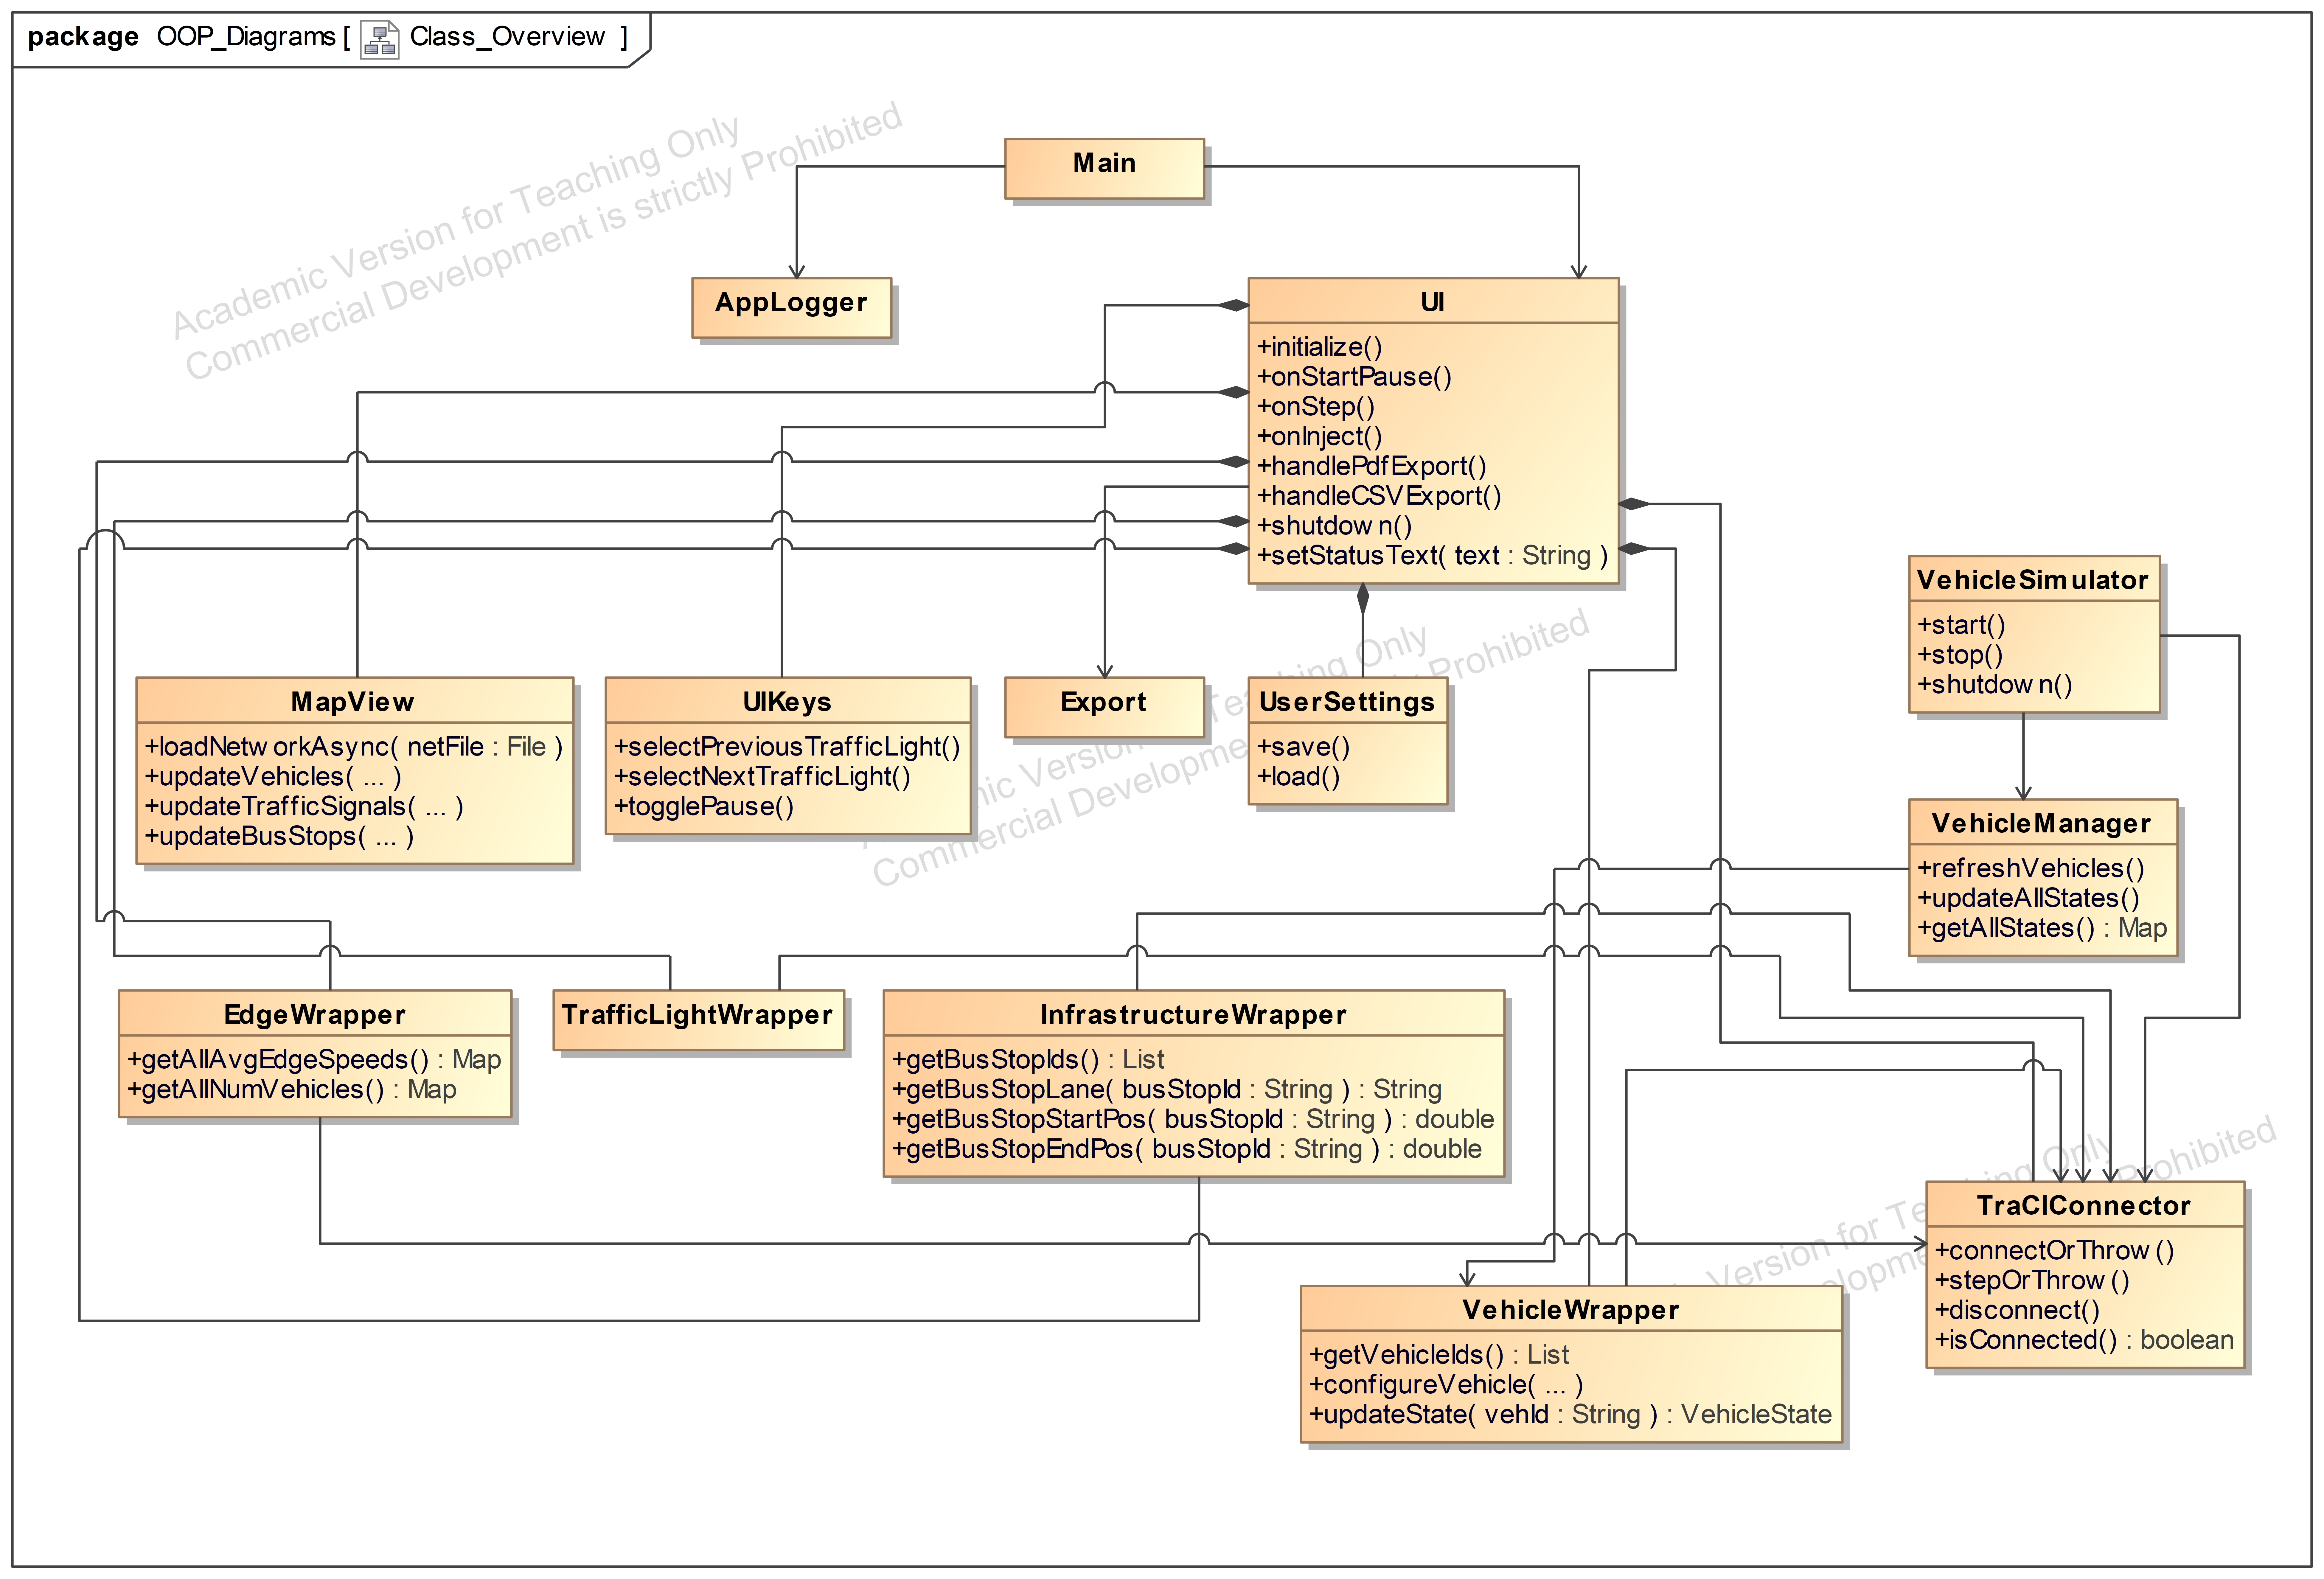
\includegraphics[width=0.8\textwidth]{Figures/Class_Overview.jpg}
	\caption{Class Diagram Overview}
	\label{fig:classdiagram}
\end{figure}

\begin{figure}[H]
	\centering
	\includegraphics[width=0.8\textwidth]{Figures/Class_TraCI.jpg}
	\caption{TraCI Class Diagram}
	\label{fig:traci-diagram}
\end{figure}

\begin{figure}[H]
	\centering
	\includegraphics[width=0.8\textwidth]{Figures/Class_UI.jpg}
	\caption{UI Class Diagram}
	\label{fig:ui-diagram}
\end{figure}

\begin{figure}[H]
	\centering
	\includegraphics[width=0.8\textwidth]{Figures/Class_SimulationRuntime.jpg}
	\caption{Simulator Class Diagram}
	\label{fig:simulator-diagram}
\end{figure}

\noindent
The \texttt{TraCIConnector} class forms the core of the system, responsible for establishing a connection to SUMO, tracking the simulation step, and providing basic operations such as \texttt{connect()}, \texttt{step()}, and obtaining simple vehicle counts. The \texttt{VehicleWrapper} and \texttt{TrafficLightWrapper} classes each hold a reference to this connector and serve as early abstractions for accessing SUMO vehicle data and traffic light information. The \texttt{Main} class simply launches the application. This structure creates a clean separation of concerns and prepares the system for more advanced TraCI functions.
\medskip

%%%%%%%%%%%%%%
\section{Use Case Diagram}

\noindent
Figure~\ref{fig:usecasediagram} presents the simplified use case diagram.
\medskip

\begin{figure}[H]
	\centering
	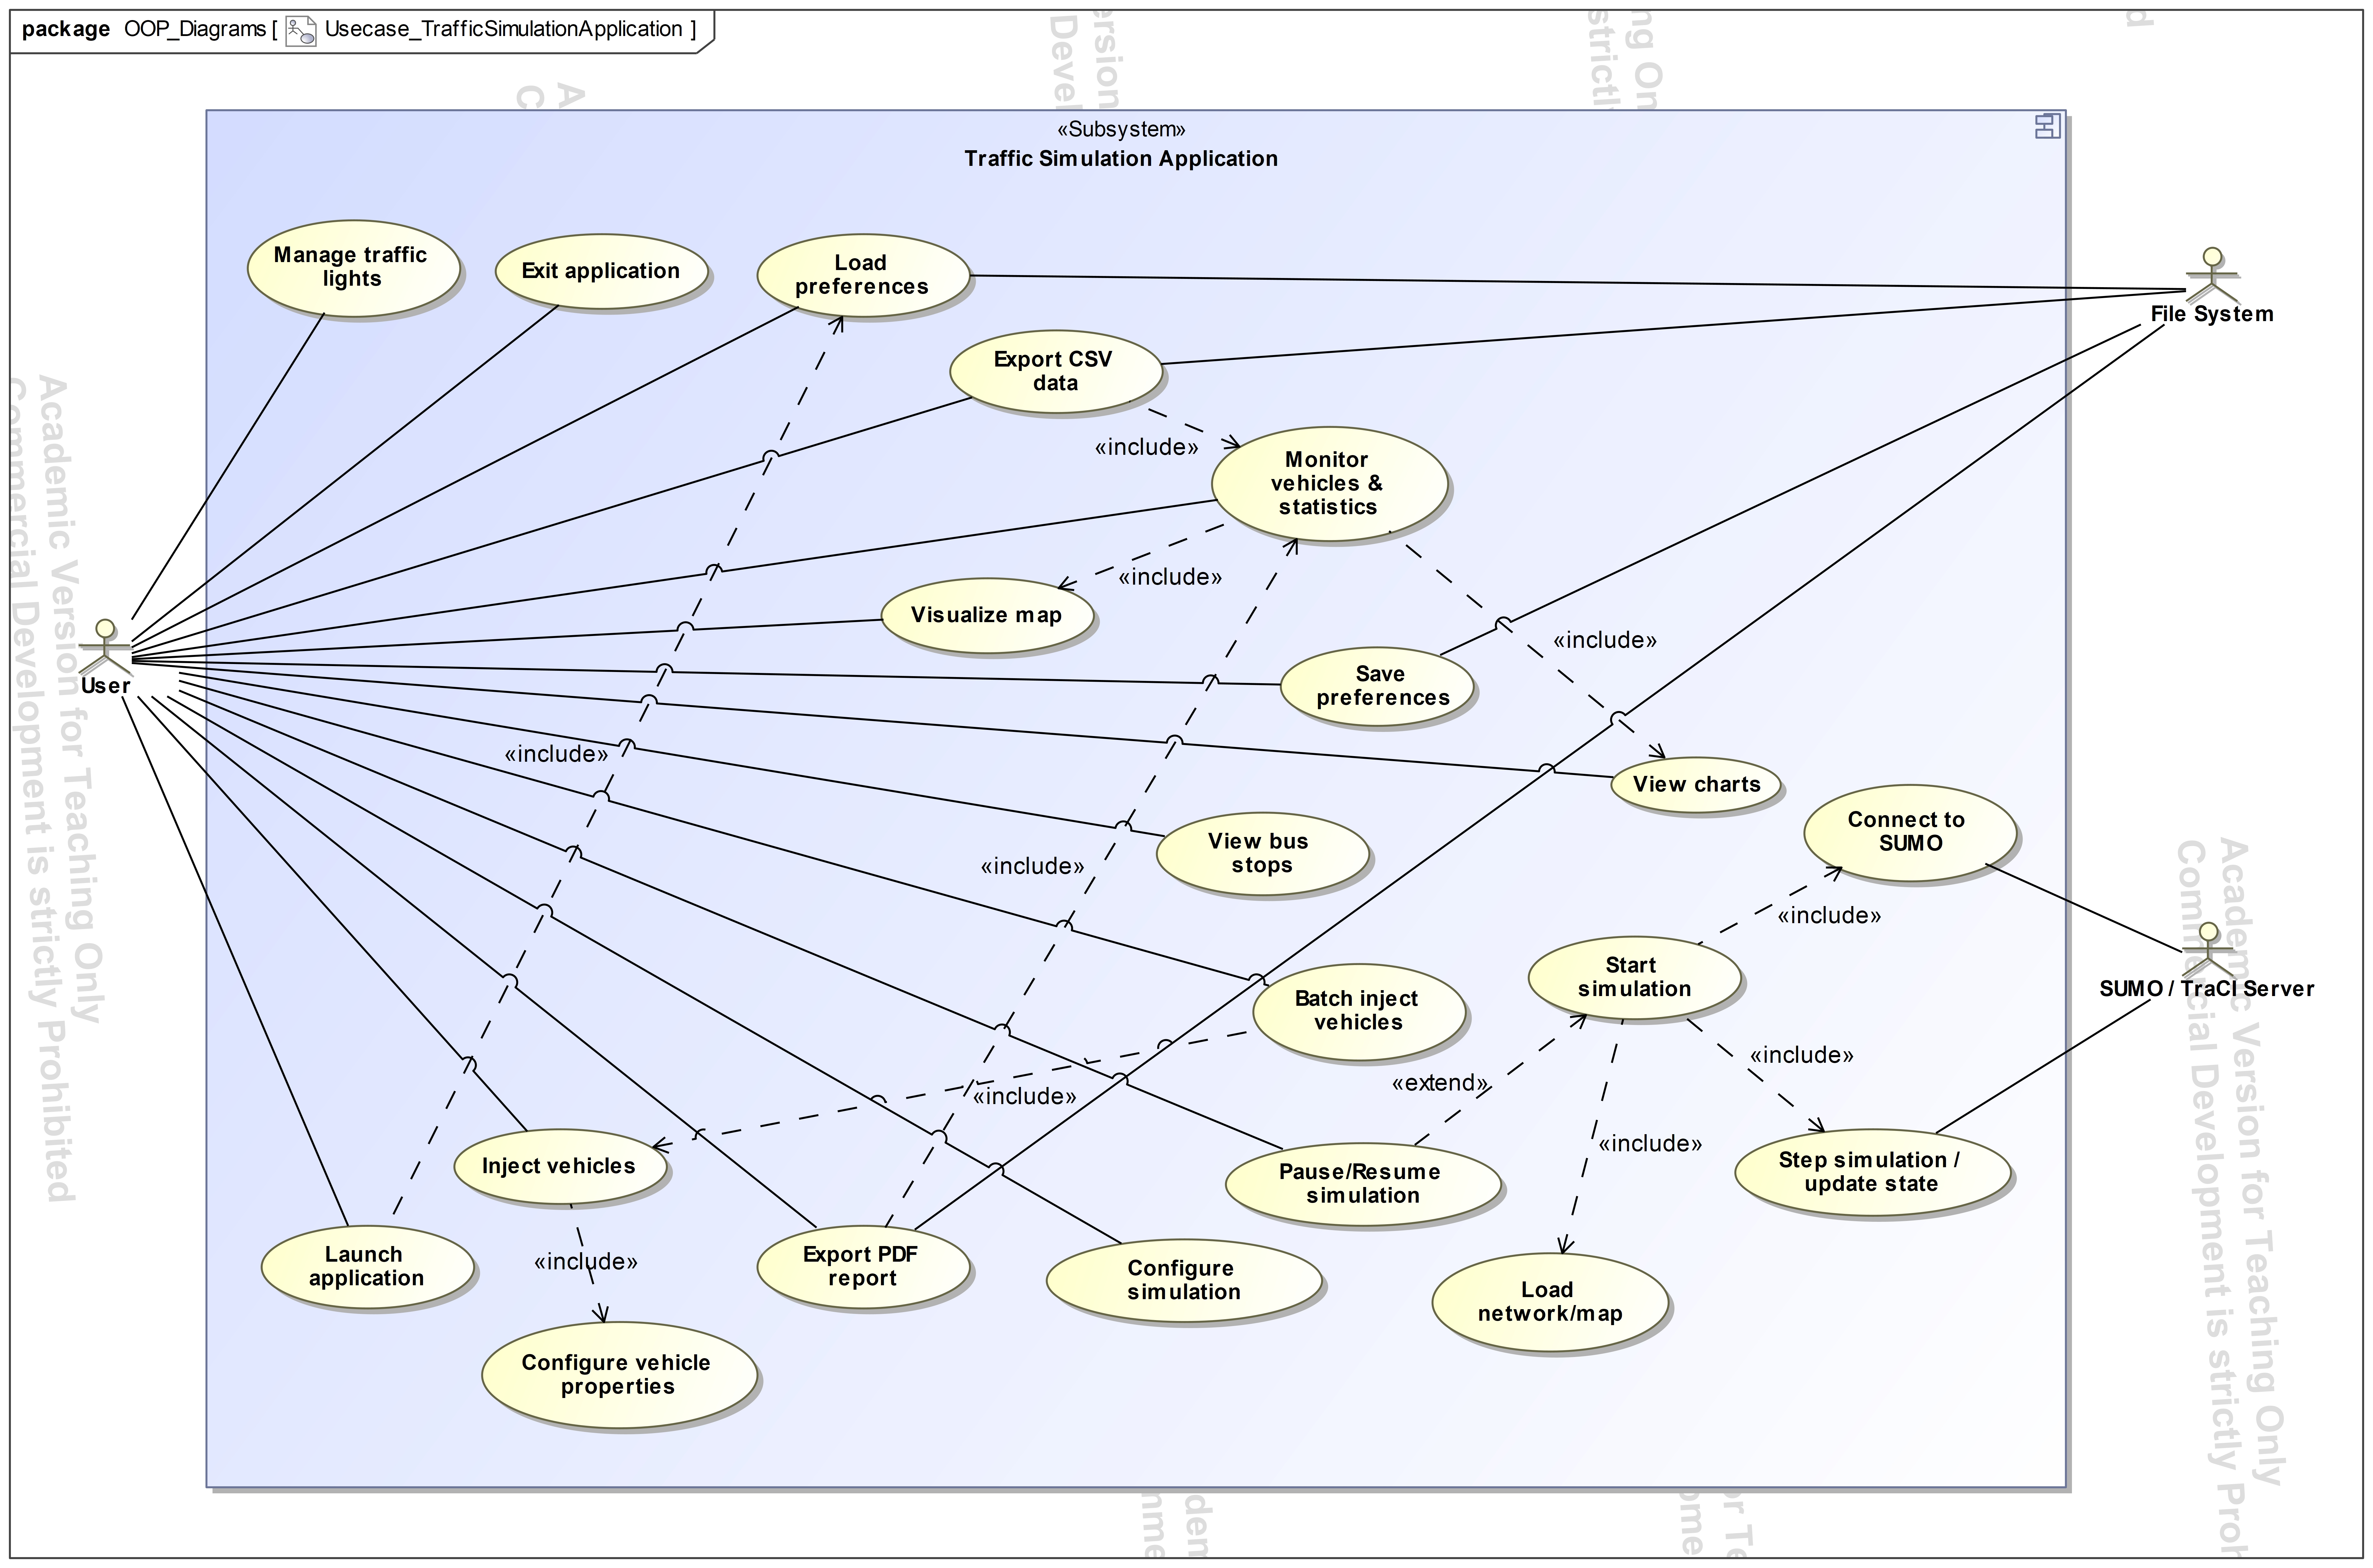
\includegraphics[width=1\textwidth]{Figures/Usecase_TrafficSimulationApplication.jpg}
	\caption{Use case diagram for the traffic simulation application}
	\label{fig:usecasediagram}
\end{figure}

\noindent
Most of the functionality here is outlined in the Core Features section. Please refer to it for more information.
\medskip

%%%%%%%%%%%%%
\section{Code Documentation and User Guide}

\noindent
Core components are documented using Javadoc and targeted inline comments, focusing on public APIs and non-trivial logic (e.g., TraCI connection lifecycle, map rendering, and vehicle state caching). A draft user guide (\texttt{userguide.md}) describes environment setup, launching the application, and the main UI workflows.
\medskip

\noindent
General documentation of the project can be found at:
\newline
\url{https://github.com/hunggiadao/realtime-traffic-simulation-java-oop/blob/main/README.md}
\medskip

\noindent
The user guide can be found at:
\newline
\url{https://github.com/hunggiadao/realtime-traffic-simulation-java-oop/blob/main/userguide.md}
\medskip

%%%%%%%%%%%%%
\section{Stress Test Scenario and Results}

\noindent
To validate the prototype under load, we prepared a stress-test scenario (\texttt{Stress.sumocfg}) that generates a high number of vehicles to stress vehicle injection, filtering, and rendering performance. This scenario was used to identify CPU-intensive parts of the update loop (map redraw and table refresh) and to motivate throttling strategies (e.g., updating the table less frequently or increasing the simulation \texttt{step-length}).
\medskip

\begin{figure}[H]
    \centering
    \includegraphics[width=0.8\textwidth]{Figures/main_ui_stress_2.png}
    \caption{Stress test run of the application with a high vehicle count.}
    \label{fig:stress-overview}
\end{figure}

%%%%%%%%%%%%%%
\section{Traffic Network Preparation}

\noindent
To test the SUMO setup during Milestone 1, we constructed a small traffic network based on a real street layout in Frankfurt. The area was selected for its moderate size and clear road geometry, making it ideal for early simulation testing. Figure \ref{fig:mapreference} shows the reference map used during the process.
\medskip

\begin{figure}[H]
    \centering
    \includegraphics[width=0.75\textwidth]{Figures/map_sample.png}
    \caption{Reference street layout used for building the SUMO network.}
    \label{fig:mapreference}
\end{figure}

\noindent
Using SUMO's NETEDIT tool, the roads, intersections, and lane connections were recreated manually. This allowed the team to produce a valid \texttt{.net.xml} file that could be loaded into SUMO for simulation.
\medskip

%%%%%%%%%
\section{SUMO Network and Initial Simulation Test}

\noindent
Once the road geometry was created in NETEDIT, the network was paired with a basic route file and loaded into SUMO for testing. Figure \ref{fig:sumosimulation} shows the SUMO GUI rendering of the test network.
\medskip

\begin{figure}[H]
	\centering
	\includegraphics[width=0.8\textwidth]{Figures/Sumo_Demo_Connection.png}
	\caption{SUMO network used for the initial simulation test}
	\label{fig:sumosimulation}
\end{figure}

\noindent
This simulation confirmed that lane connections, turning paths, and traffic flow behaved as expected. The successful run ensured that the SUMO environment, map setup, and route files were correctly prepared for Java integration in later phases.
\medskip

%%%%%%%%%%%%%%
\section{TraCI Connection Test}

\noindent
During Milestone~1, we performed a small integration test to verify that a Java application could successfully communicate with SUMO via TraCI. 
\medskip

\noindent
The connector established a SUMO process, stepped the simulation once, and retrieved a simple vehicle count, confirming a working communication pipeline. Figure~\ref{fig:tracitest} illustrates the demo used during testing.
\medskip

\begin{figure}[H]
    \centering
    \includegraphics[width=1\textwidth]{Figures/sumo_connection_test.png}
    \caption{Demo of the Java--SUMO TraCI connection during Milestone~1.}
    \label{fig:tracitest}
\end{figure}

\noindent
This confirms that the communication layer works and can be expanded with more detailed functions in the next milestones.
\medskip
